\section{Final remarks}

The $n$-tree comparison is a necessary condition on the finite metric space which admits an isometric embedding into a nonnegatively curved Alexandrov space.
This condition is not sufficient for metric spaces with at least 6 points;
the corresponding example was constructed by Sergei Ivanov, see \cite{AKP}.

Theorem~\ref{2(2)+3(1)}, provides a source for such examples --- it is sufficient to construct construct 6-pint metric space which satisfy all 5-tree comparisons, but does not satisfy 2(2)-tree comparison.

We expect that the comparisons for trees 5 and 2(2) (the two trees on the diagram) are sufficient. 
\hide
\begin{center}
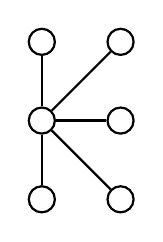
\begin{tikzpicture}[scale=1,
  thick,main node/.style={circle,draw,font=\sffamily\bfseries,minimum size=3mm}]

  \node[main node] (1) at (0,0) {};
  \node[main node] (2) at (0,1){};
  \node[main node] (3) at (0,2){};
  \node[main node] (4) at (1,0) {};
  \node[main node] (5) at (1,1) {};
  \node[main node] (6) at (1,2) {};

  \path[every node/.style={font=\sffamily\small}]
   (1) edge node[above]{}(2)
   (2) edge node[above]{}(3)
   (2) edge node[above]{}(4)
   (2) edge node[above]{}(5)
   (2) edge node[above]{}(6);
\end{tikzpicture}
\hskip10mm
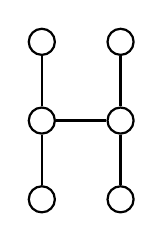
\begin{tikzpicture}[scale=1,
  thick,main node/.style={circle,draw,font=\sffamily\bfseries,minimum size=3mm}]

  \node[main node] (1) at (0,0) {};
  \node[main node] (2) at (0,1){};
  \node[main node] (3) at (0,2){};
  \node[main node] (4) at (1,0) {};
  \node[main node] (5) at (1,1) {};
  \node[main node] (6) at (1,2) {};

  \path[every node/.style={font=\sffamily\small}]
   (1) edge node[above]{}(2)
   (2) edge node[above]{}(3)
   (2) edge node[above]{}(5)
   (5) edge node[above]{}(6)
   (4) edge node[above]{}(5);
\end{tikzpicture}
\end{center}
\unhide

For 5-point metric spaces the 4-comparisons should be sufficient.